\documentclass{article}
\usepackage{ctex}
\usepackage{graphicx}
\usepackage{listings}
\usepackage{xcolor}
\usepackage{geometry}
\usepackage{amsmath}
\usepackage{titling}
\usepackage{ragged2e}

% 页面设置
\geometry{a4paper, margin=2.5cm}
% 代码高亮设置
\lstset{
    language=Matlab,
    backgroundcolor=\color{gray!10},
    basicstyle=\ttfamily\small,
    keywordstyle=\color{blue},
    commentstyle=\color{green!70},
    stringstyle=\color{red},
    frame=single,
    breaklines=true,
    numbers=left,
    numberstyle=\tiny,
    captionpos=b,
    escapeinside={/*@}{@*/}
}

\begin{document}

% ====================== 抄袭警示声明 ======================
\begin{center}
\vspace*{2cm}
\Large\textbf{\color{red}⚠️ 重要声明}

\vspace{0.8cm}
\large
本文档仅作为学习思路、代码原理参考资料。\\
严禁直接复制全文提交作为个人实验报告，抄袭会造成课程成绩失效、学术不端处分。\\
请自主理解原理、修改代码与行文，独立完成实验报告。

\vspace{1.5cm}
\rule{0.6\textwidth}{0.6pt}
\vspace{3cm}
\end{center}

% ---------------------- 哈工大（深圳）封面 ----------------------
\begin{titlepage}
    \centering
    % 顶部学校名称
    \Huge{\textbf{哈尔滨工业大学（深圳）}}\\
    \vspace{0.5cm}
    \Large{\textbf{电磁场实验报告}}\\
    \vspace{2cm}
    
    % 实验名称
    \huge{\textbf{静电场有限差分法编程实现}}\\
    \vspace{3cm}
    
    % 信息表格（移除班级、姓名、学号）
    \large
    \begin{tabular}{ll}
        \textbf{课程名称：} & \quad 电磁场 \\
        \textbf{实验名称：} & \quad 实验一 有限差分法求解二维静电场 \\
        \textbf{完成日期：} & \quad 2026年05月09日 \\
    \end{tabular}
    
    \vfill
    \small{\textit{Harbin Institute of Technology, Shenzhen}}
\end{titlepage}

% ---------------------- 正文内容 ----------------------
\section{实验题图}
\begin{center}
    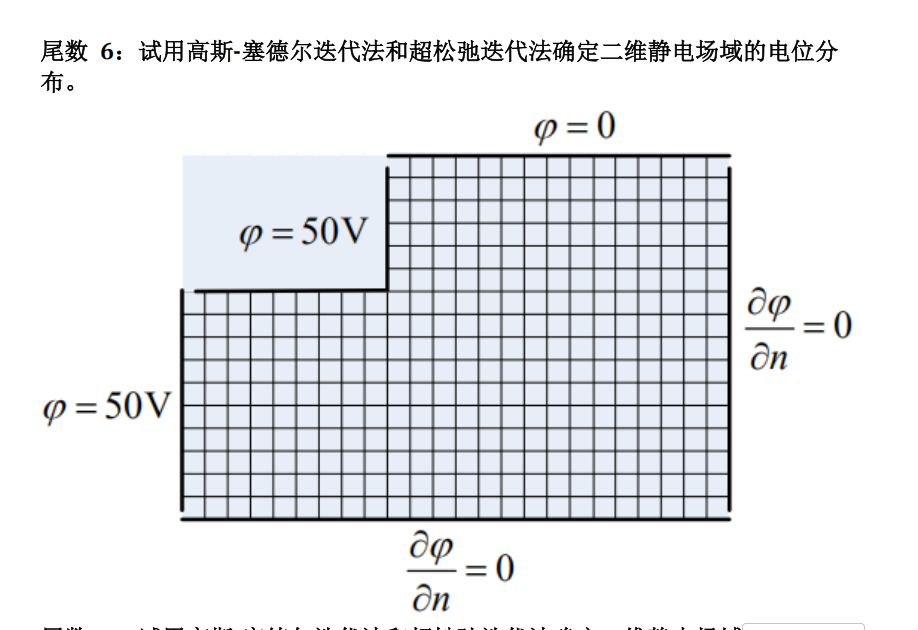
\includegraphics[width=0.6\textwidth]{题目.png}
\end{center}

\section{实验程序}
\begin{lstlisting}[caption=MATLAB 求解二维静电场有限差分迭代程序]
% ==============================
% 二维静电场求解：SOR迭代 + 高斯-赛德尔迭代 尾号06
% ==============================
clear; clc; close all;

% 公共参数
hx=25;hy=17; %设置网格节点数
m=24;n=16;%横纵向网格数

%% ====================== 一、高斯-赛德尔迭代法 ======================
disp('==================== 高斯-赛德尔迭代结果 ====================');
v_gs=ones(hy,hx);
v_gs(1:6,17:25)=zeros(6,9);
% Dirichlet 边界条件
v_gs(1,10:25)=0;
v_gs(2:7,10)=50;
v_gs(7,1:10)=50;
v_gs(7:16,1)=50;

v2_gs = v_gs;
maxt=1;
k_gs=0;

while(maxt>1e-6)
    k_gs=k_gs+1;
    maxt=0;
    v_old = v2_gs;
    
    % 上区域迭代
    for i=2:7
        for j=11:24
            v2_gs(i,j) = (v2_gs(i,j+1)+v2_gs(i+1,j)+v2_gs(i-1,j)+v2_gs(i,j-1))/4;
            t=abs(v2_gs(i,j)-v_old(i,j));
            if(t>maxt) maxt=t;end
        end
    end
    % 下区域迭代
    for i=8:(hy-1)
        for j=2:(hx-1)
            v2_gs(i,j) = (v2_gs(i,j+1)+v2_gs(i+1,j)+v2_gs(i-1,j)+v2_gs(i,j-1))/4;
            t=abs(v2_gs(i,j)-v_old(i,j));
            if(t>maxt) maxt=t;end
        end
    end
    
    % Neumann 边界条件：右、下偏导为0
    v2_gs(7:hy-1,hx)=v2_gs(7:hy-1,hx-1);
    v2_gs(hy,1:hx)=v2_gs(hy-1,1:hx);
end

% 输出高斯-赛德尔结果
fprintf('高斯-赛德尔迭代次数：%d\n',k_gs);
disp('高斯-赛德尔最终电位矩阵：');
disp(v2_gs);
v_gs_plot = v2_gs(hy:-1:1,:);

%% ====================== 二、SOR超松弛迭代法 ======================
disp('==================== SOR超松弛迭代结果 ====================');
v1=ones(hy,hx);
v1(1:6,17:25)=zeros(6,9);
%边界的 Dirichlet 边界条件值
v1(1,10:25)=ones(1,16)*0;
v1(2:7,10)=ones(6,1)*50;
v1(7,1:10)=ones(1,10)*50;
v1(7:16,1)=50;

%计算松弛因子
t1=(cos(pi/m)+cos(pi/n))/2;
w=2/(1+sqrt(1-t1*t1));
v2=v1;maxt=1;t=0;%初始化
k=0;
while(maxt>1e-6)%由 v1 迭代，算出 v2，迭代精度为 0.000001
    k=k+1;%计算迭代次数
    maxt=0;
    for i=2:7%从 2 到 7 行循环
        for j=11:24%从 2 到 15 列循环
            v2(i,j)=v1(i,j)+(v1(i,j+1)+v1(i+1,j)+v2(i-1,j)+v2(i,j-1)-4*v1(i,j))*w/4;%拉普拉斯方程差分式
            t=abs(v2(i,j)-v1(i,j));
            if(t>maxt) maxt=t;end
        end
    end
    for i=8:(hy-1)%从 8 到 hy-1 行循环
        for j=2:(hx-1)%从 2 到 hx-1 列循环
            v2(i,j)=v1(i,j)+(v1(i,j+1)+v1(i+1,j)+v2(i-1,j)+v2(i,j-1)-4*v1(i,j))*w/4;%拉普拉斯方程差分式
            t=abs(v2(i,j)-v1(i,j));
            if(t>maxt) maxt=t;end
        end
    end
    % 最右侧边界 偏导为0 Neumann边界条件
    v2(7:hy-1,hx)=v2(7:hy-1,hx-1);
    % 最下侧边界 偏导为0 Neumann边界条件
    v2(hy,1:hx)=v2(hy-1,1:hx);
    v1=v2;
end
v1=v2(hy:-1:1,:);
% 输出迭代收敛后的最终电位矩阵
fprintf('SOR迭代次数：%d\n',k);
disp('SOR迭代最终电位矩阵：');
disp(v2);

%% ====================== 三、统一绘图对比 ======================
figure('Position',[100,100,1000,800]);

% 上排：高斯-赛德尔
subplot(2,2,1),mesh(v_gs_plot)
axis([0,25,0,17,0,100])
title('高斯-赛德尔 - 三维电位分布')
subplot(2,2,2),contour(v_gs_plot,50)
hold on
[xx,yy]=meshgrid(1:hx,1:hy);
[Gx,Gy]=gradient(v_gs_plot,0.6,0.6);
quiver(xx,yy,Gx,Gy,'r')
axis([-1.5,hx+2.5,-2,20])
plot([1,1,hx,hx,1],[1,hy,hy,1,1],'k')
text(hx/2-0.5,hy+0.4,'0V','fontsize',11);
text(hx/2,0.3,'\partial\phi/\partialn=0','fontsize',11);
text(-0.3,hy/2,'50V','fontsize',11);
text(hx+0.1,hy/2,'\partial\phi/\partialn=0','fontsize',11);
text(hx/2-8,hy/2+6,'50V','fontsize',11);
title('高斯-赛德尔 - 等电位线&电场')
hold off

% 下排：SOR迭代
subplot(2,2,3),mesh(v1)
axis([0,25,0,17,0,100])
title('SOR超松弛 - 三维电位分布')
subplot(2,2,4),contour(v1,50)
hold on
[Gx,Gy]=gradient(v1,0.6,0.6);
quiver(xx,yy,Gx,Gy,'r')
axis([-1.5,hx+2.5,-2,20])
plot([1,1,hx,hx,1],[1,hy,hy,1,1],'k')
text(hx/2-0.5,hy+0.4,'0V','fontsize',11);
text(hx/2,0.3,'\partial\phi/\partialn=0','fontsize',11);
text(-0.3,hy/2,'50V','fontsize',11);
text(hx+0.1,hy/2,'\partial\phi/\partialn=0','fontsize',11);
text(hx/2-8,hy/2+6,'50V','fontsize',11);
title('SOR超松弛 - 等电位线&电场')
hold off
\end{lstlisting}

\section{实验结果}
\begin{center}
    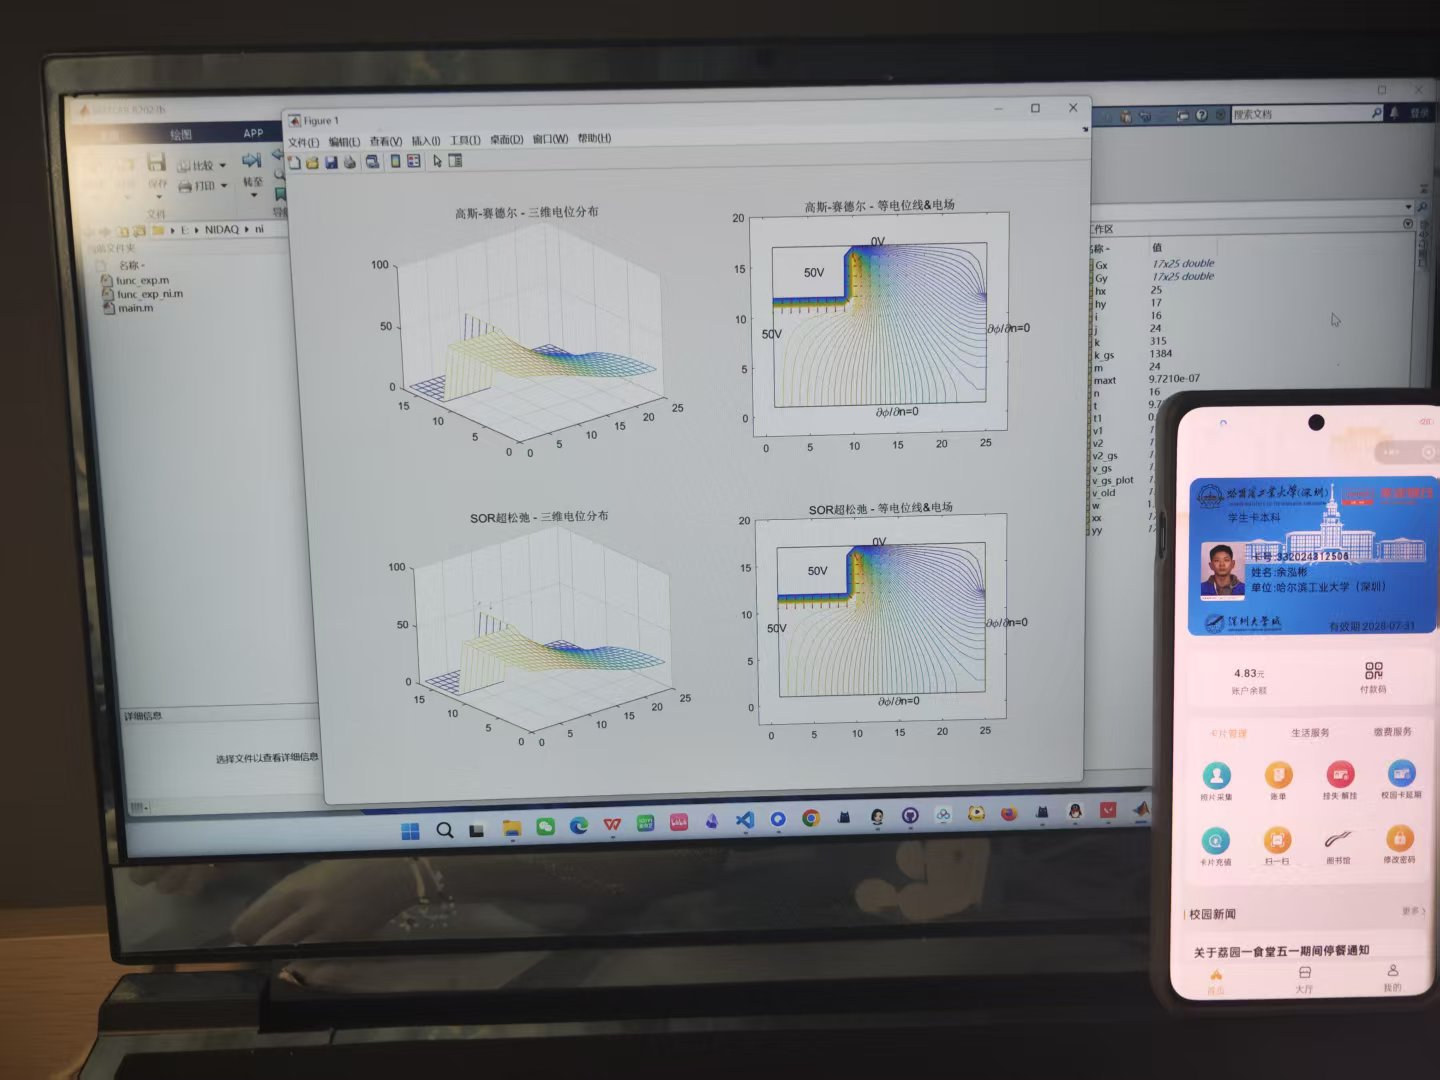
\includegraphics[width=0.85\textwidth]{1.jpg}
\end{center}
\begin{center}
    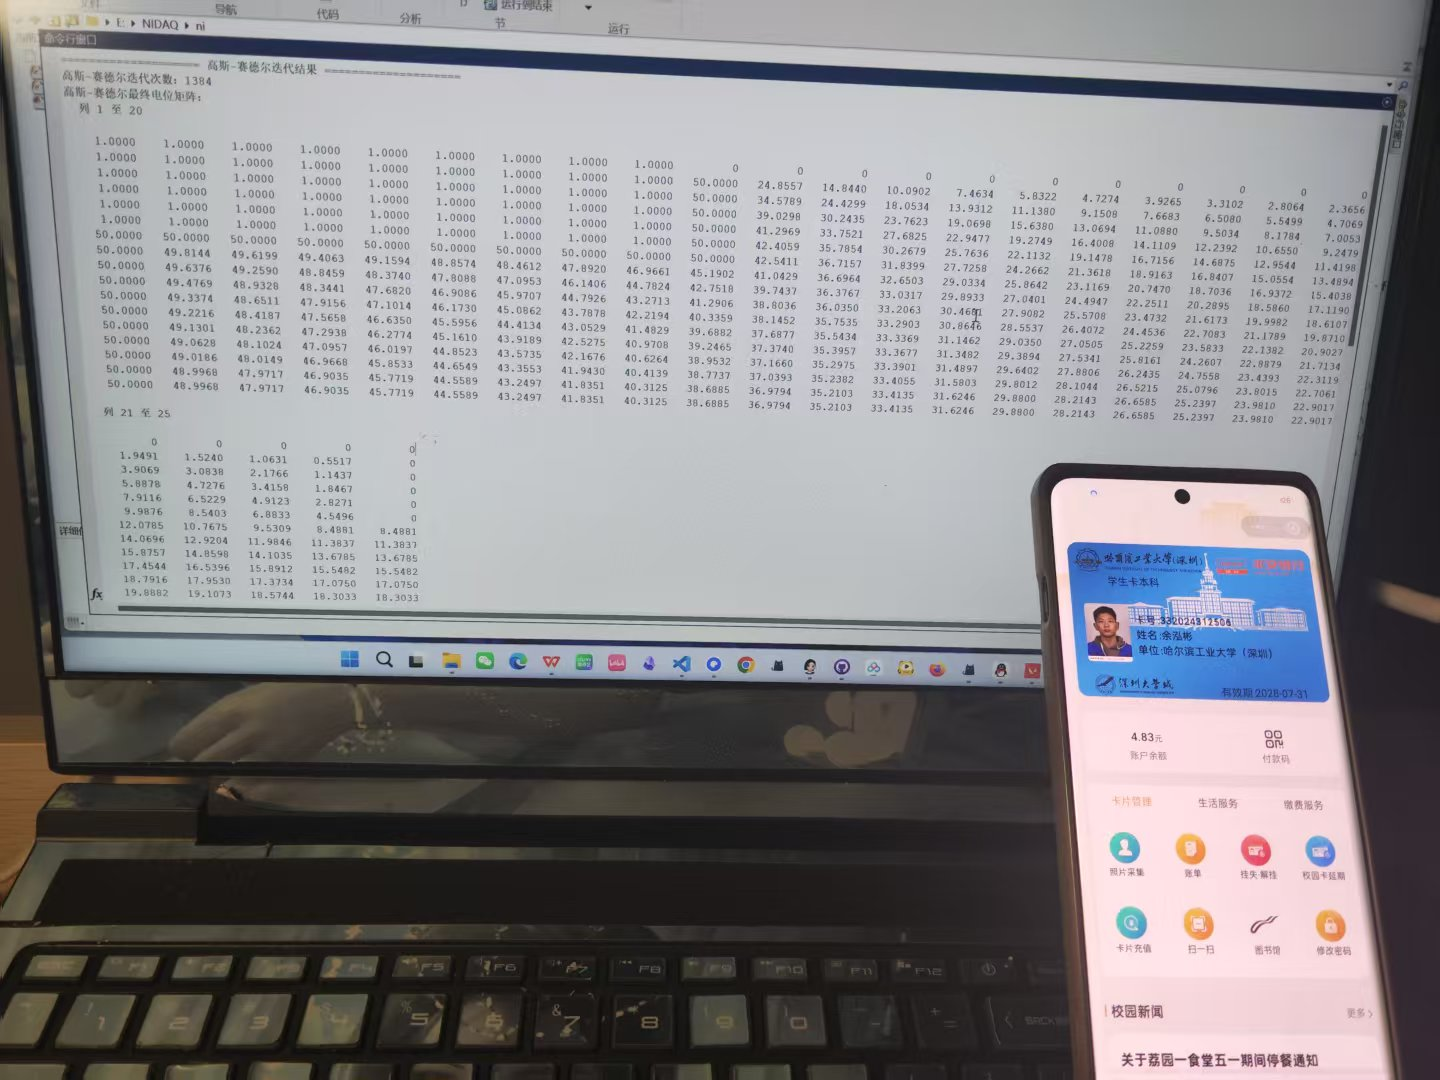
\includegraphics[width=0.85\textwidth]{2.jpg}
\end{center}
\begin{center}
    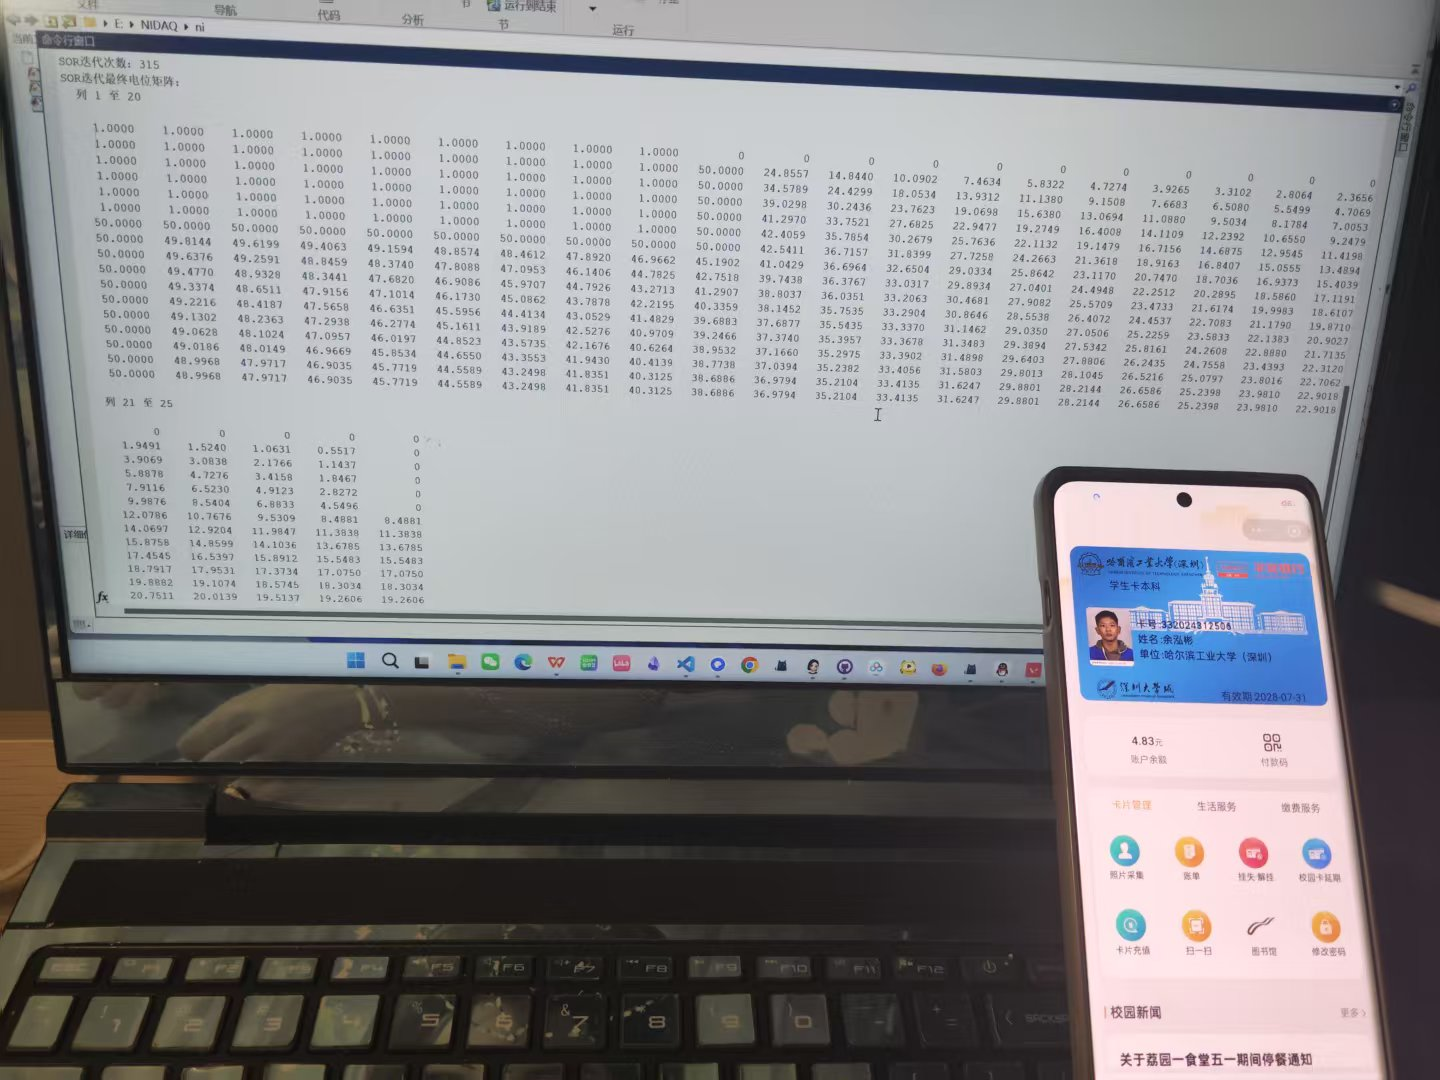
\includegraphics[width=0.85\textwidth]{3.jpg}
\end{center}

\begin{center}
    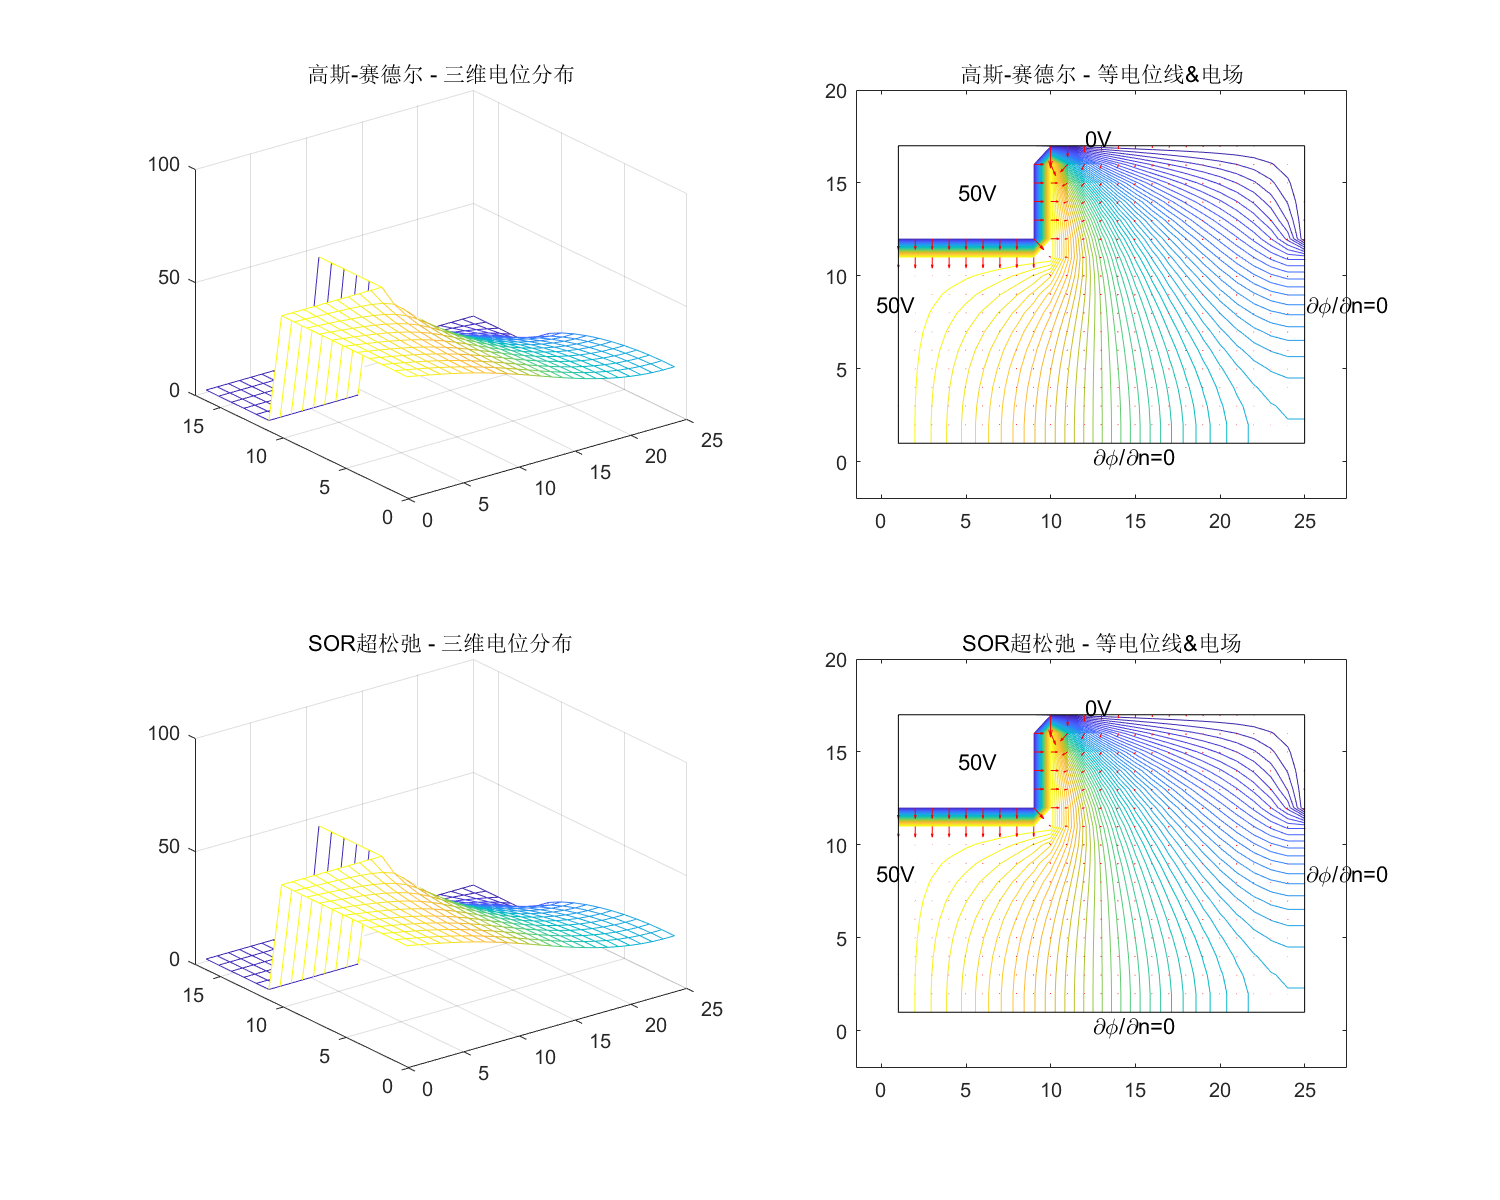
\includegraphics[width=0.85\textwidth]{结果图.png}
\end{center}

\subsection{迭代输出与电位矩阵数据}
\begin{center}
    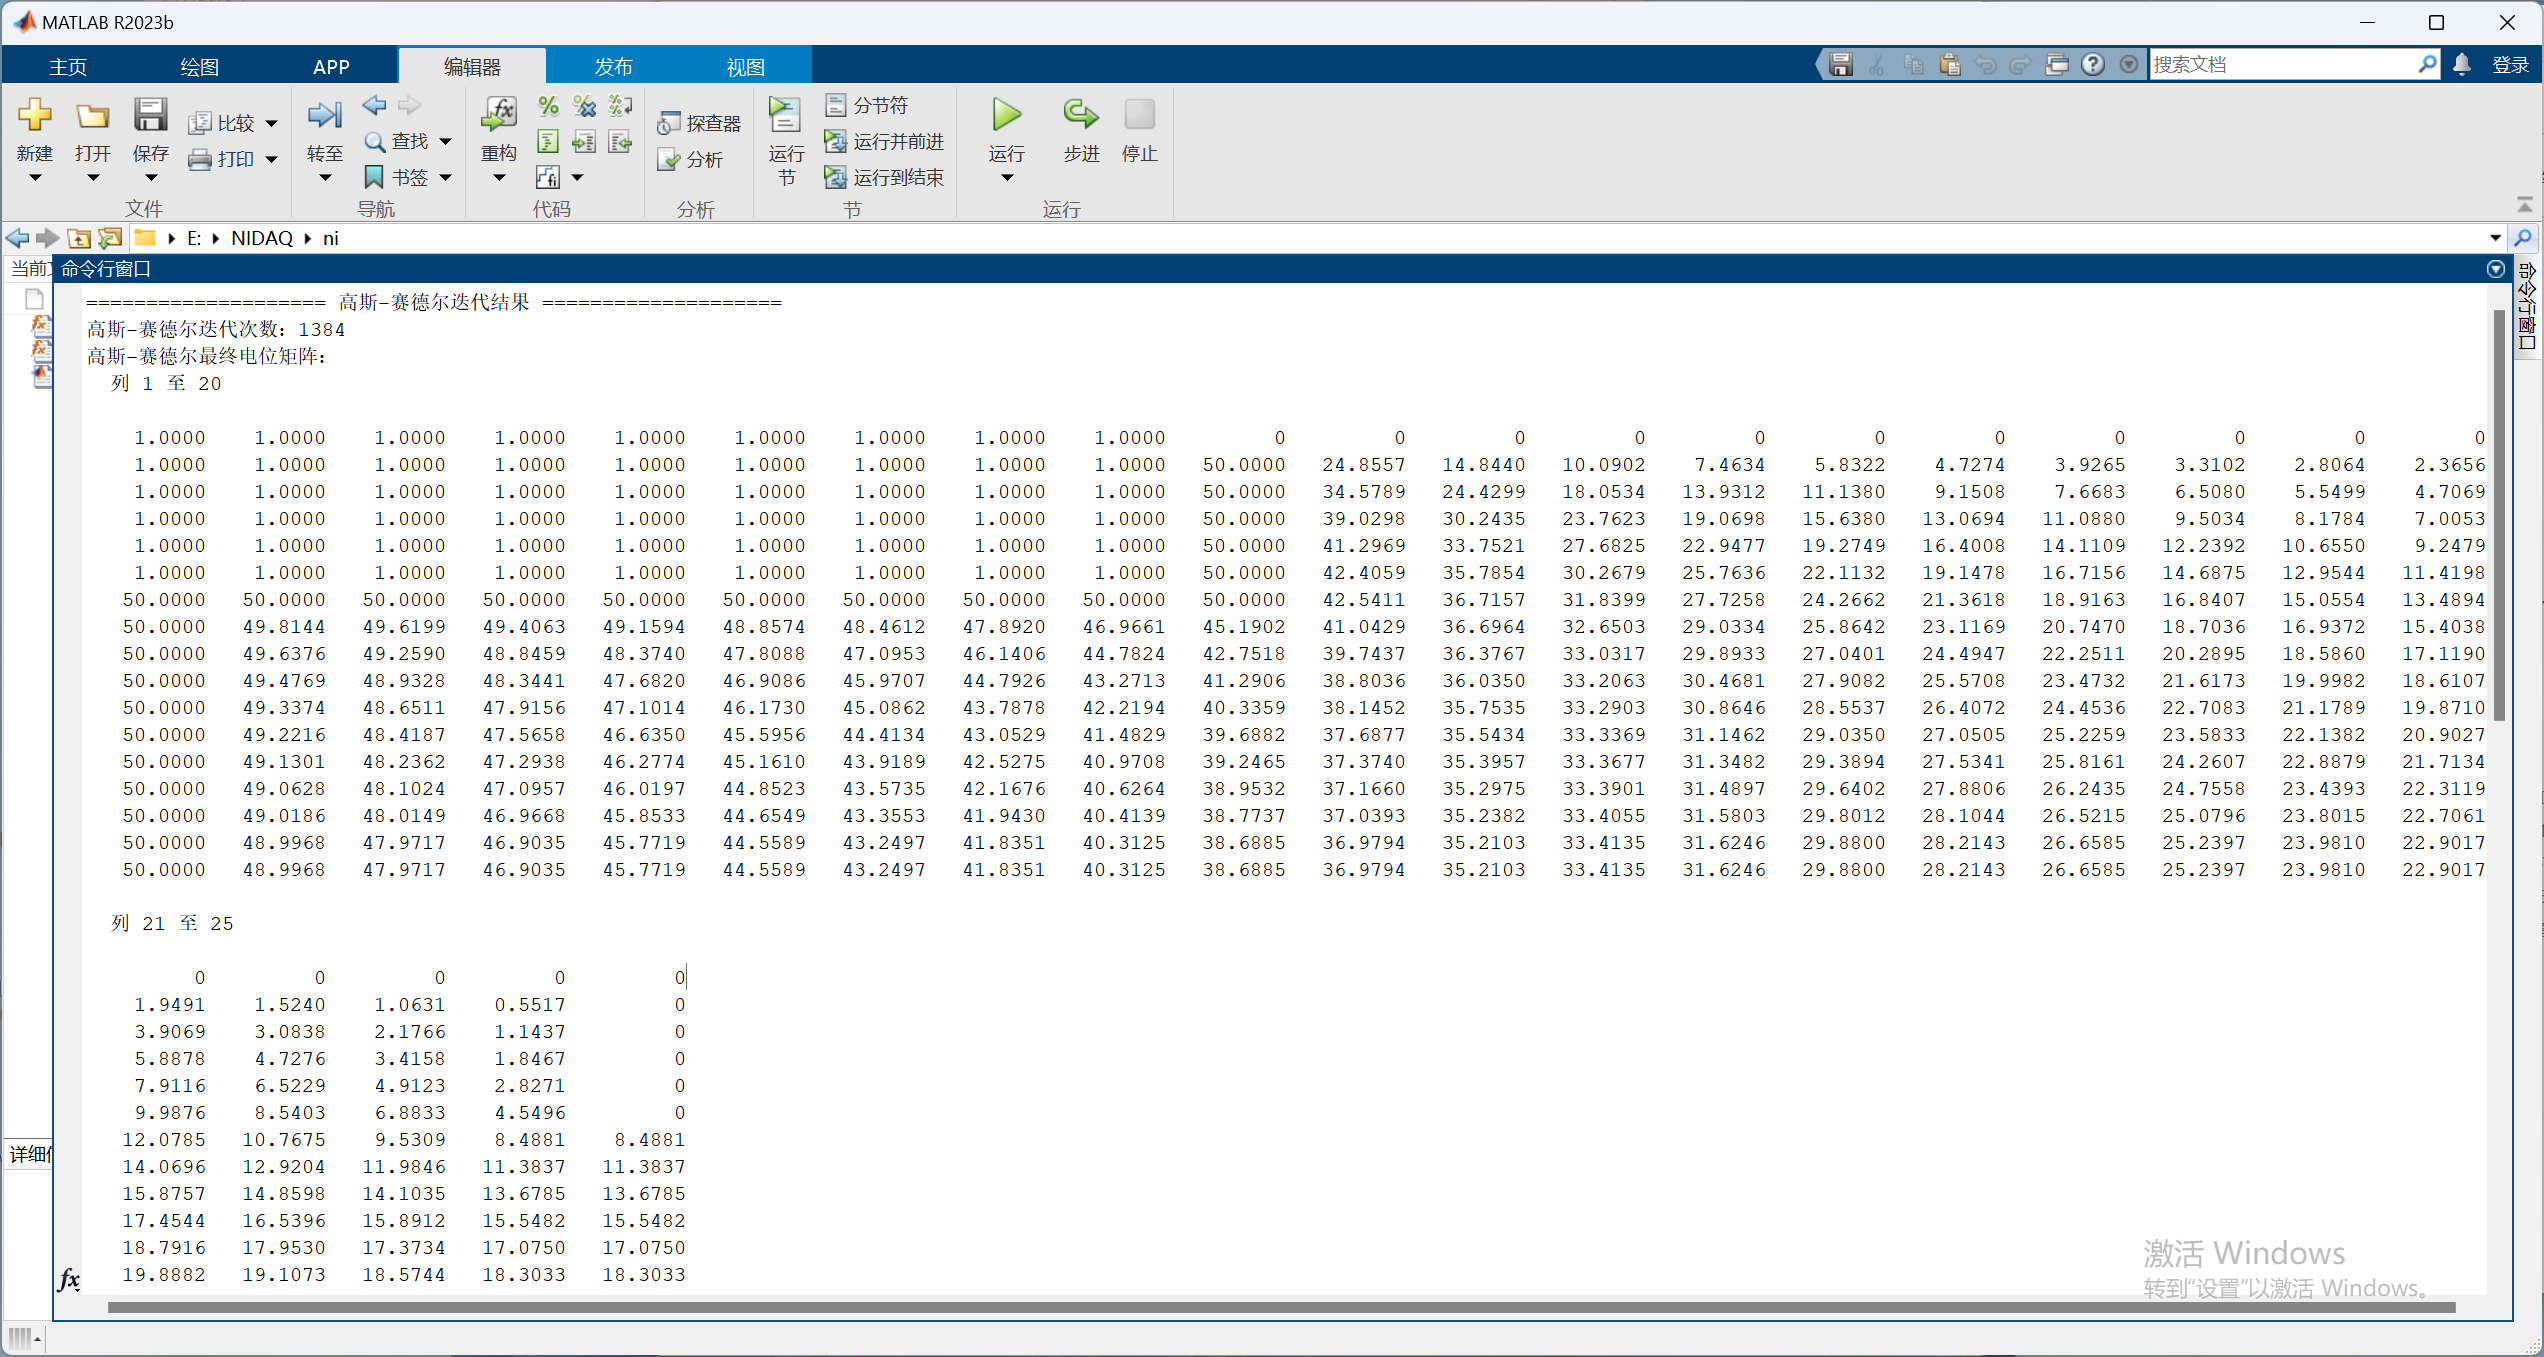
\includegraphics[width=0.85\textwidth]{数据1.png}
\end{center}
\begin{center}
    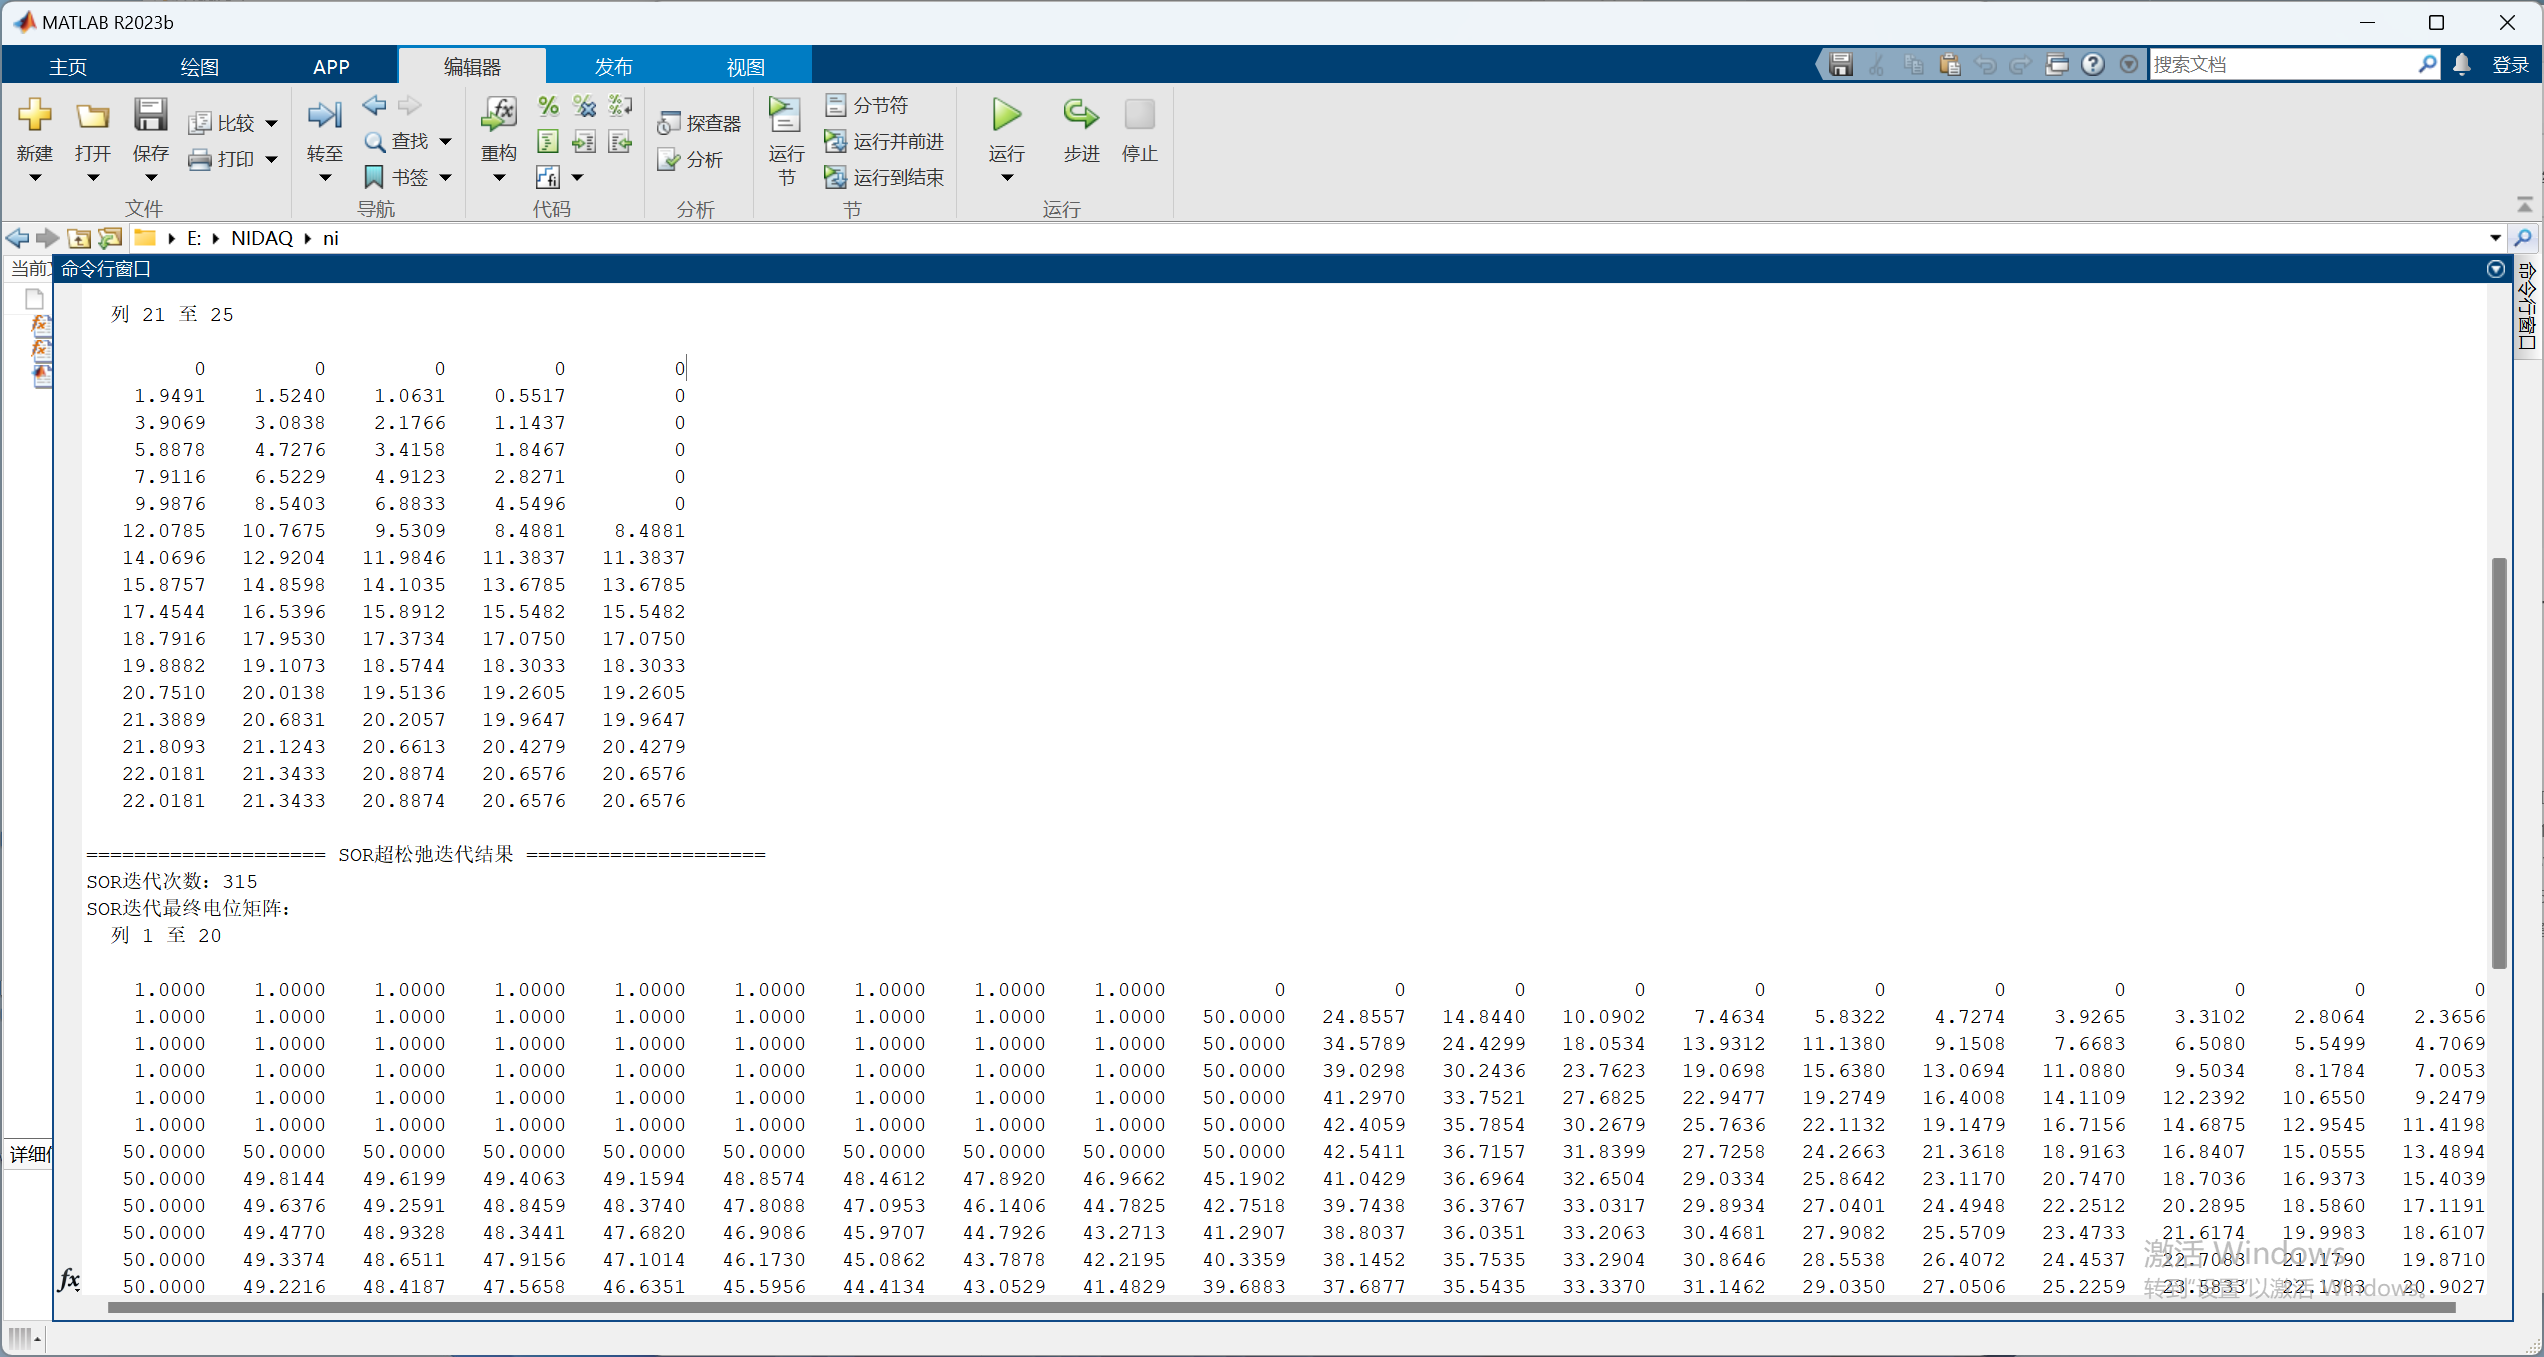
\includegraphics[width=0.85\textwidth]{数据2.png}
\end{center}
\begin{center}
    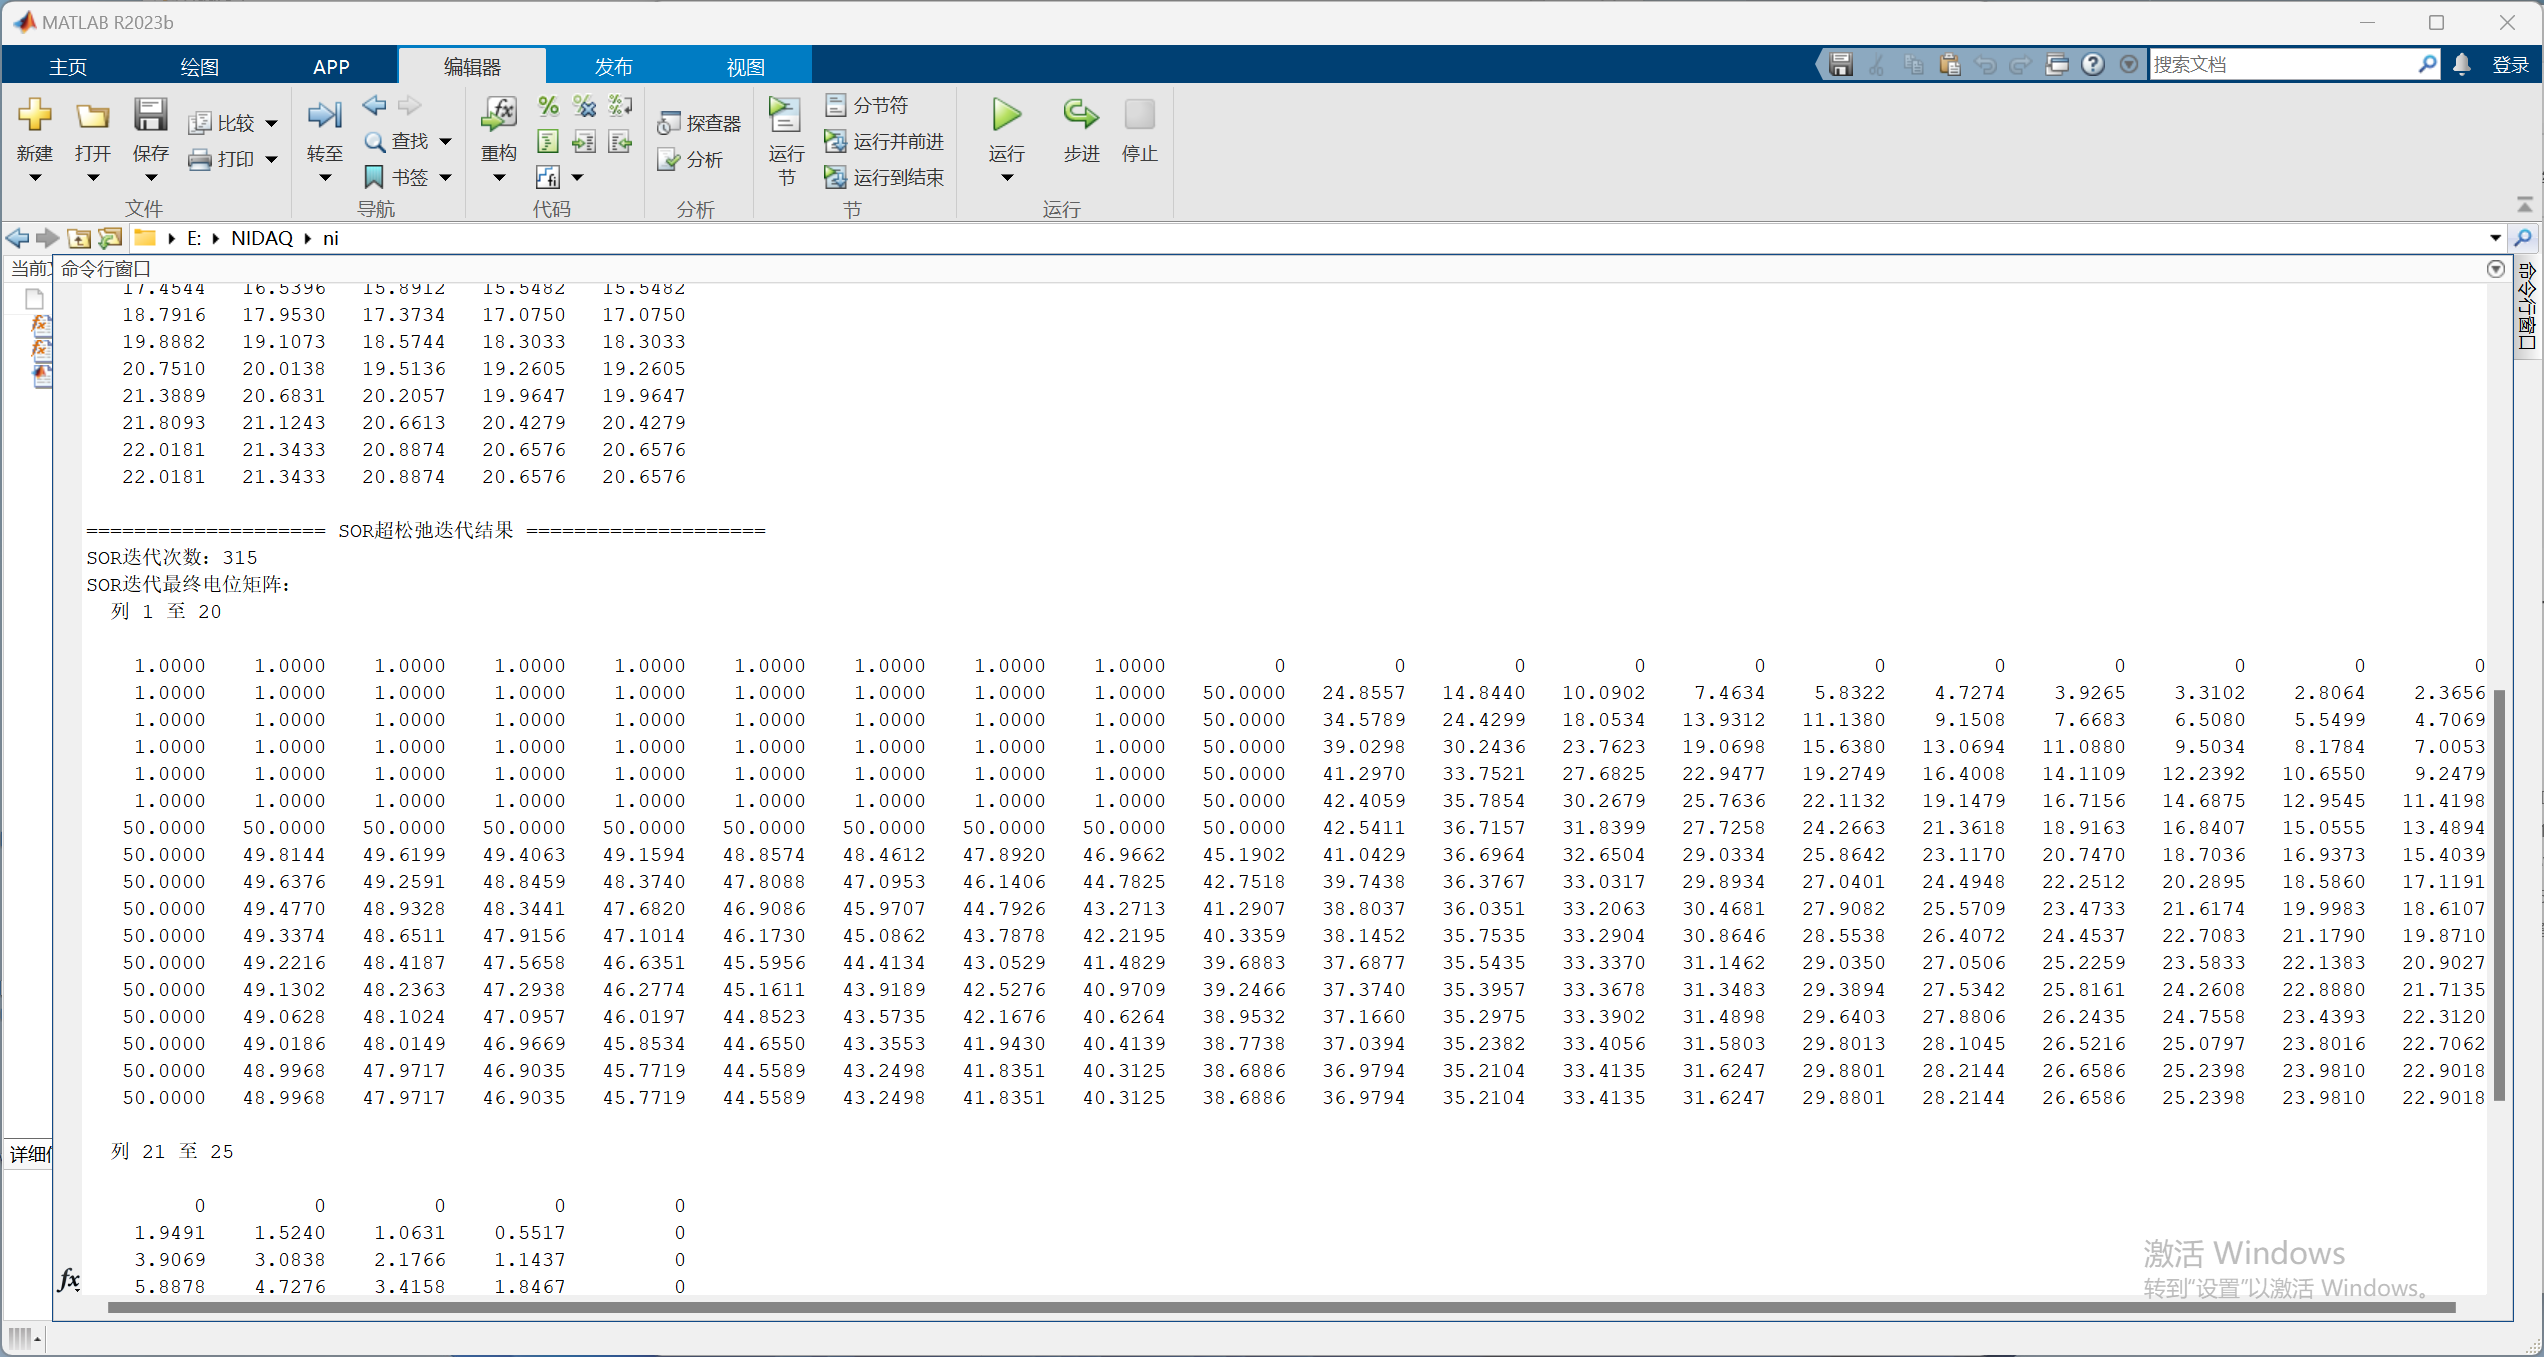
\includegraphics[width=0.85\textwidth]{数据3.png}
\end{center}
\begin{center}
    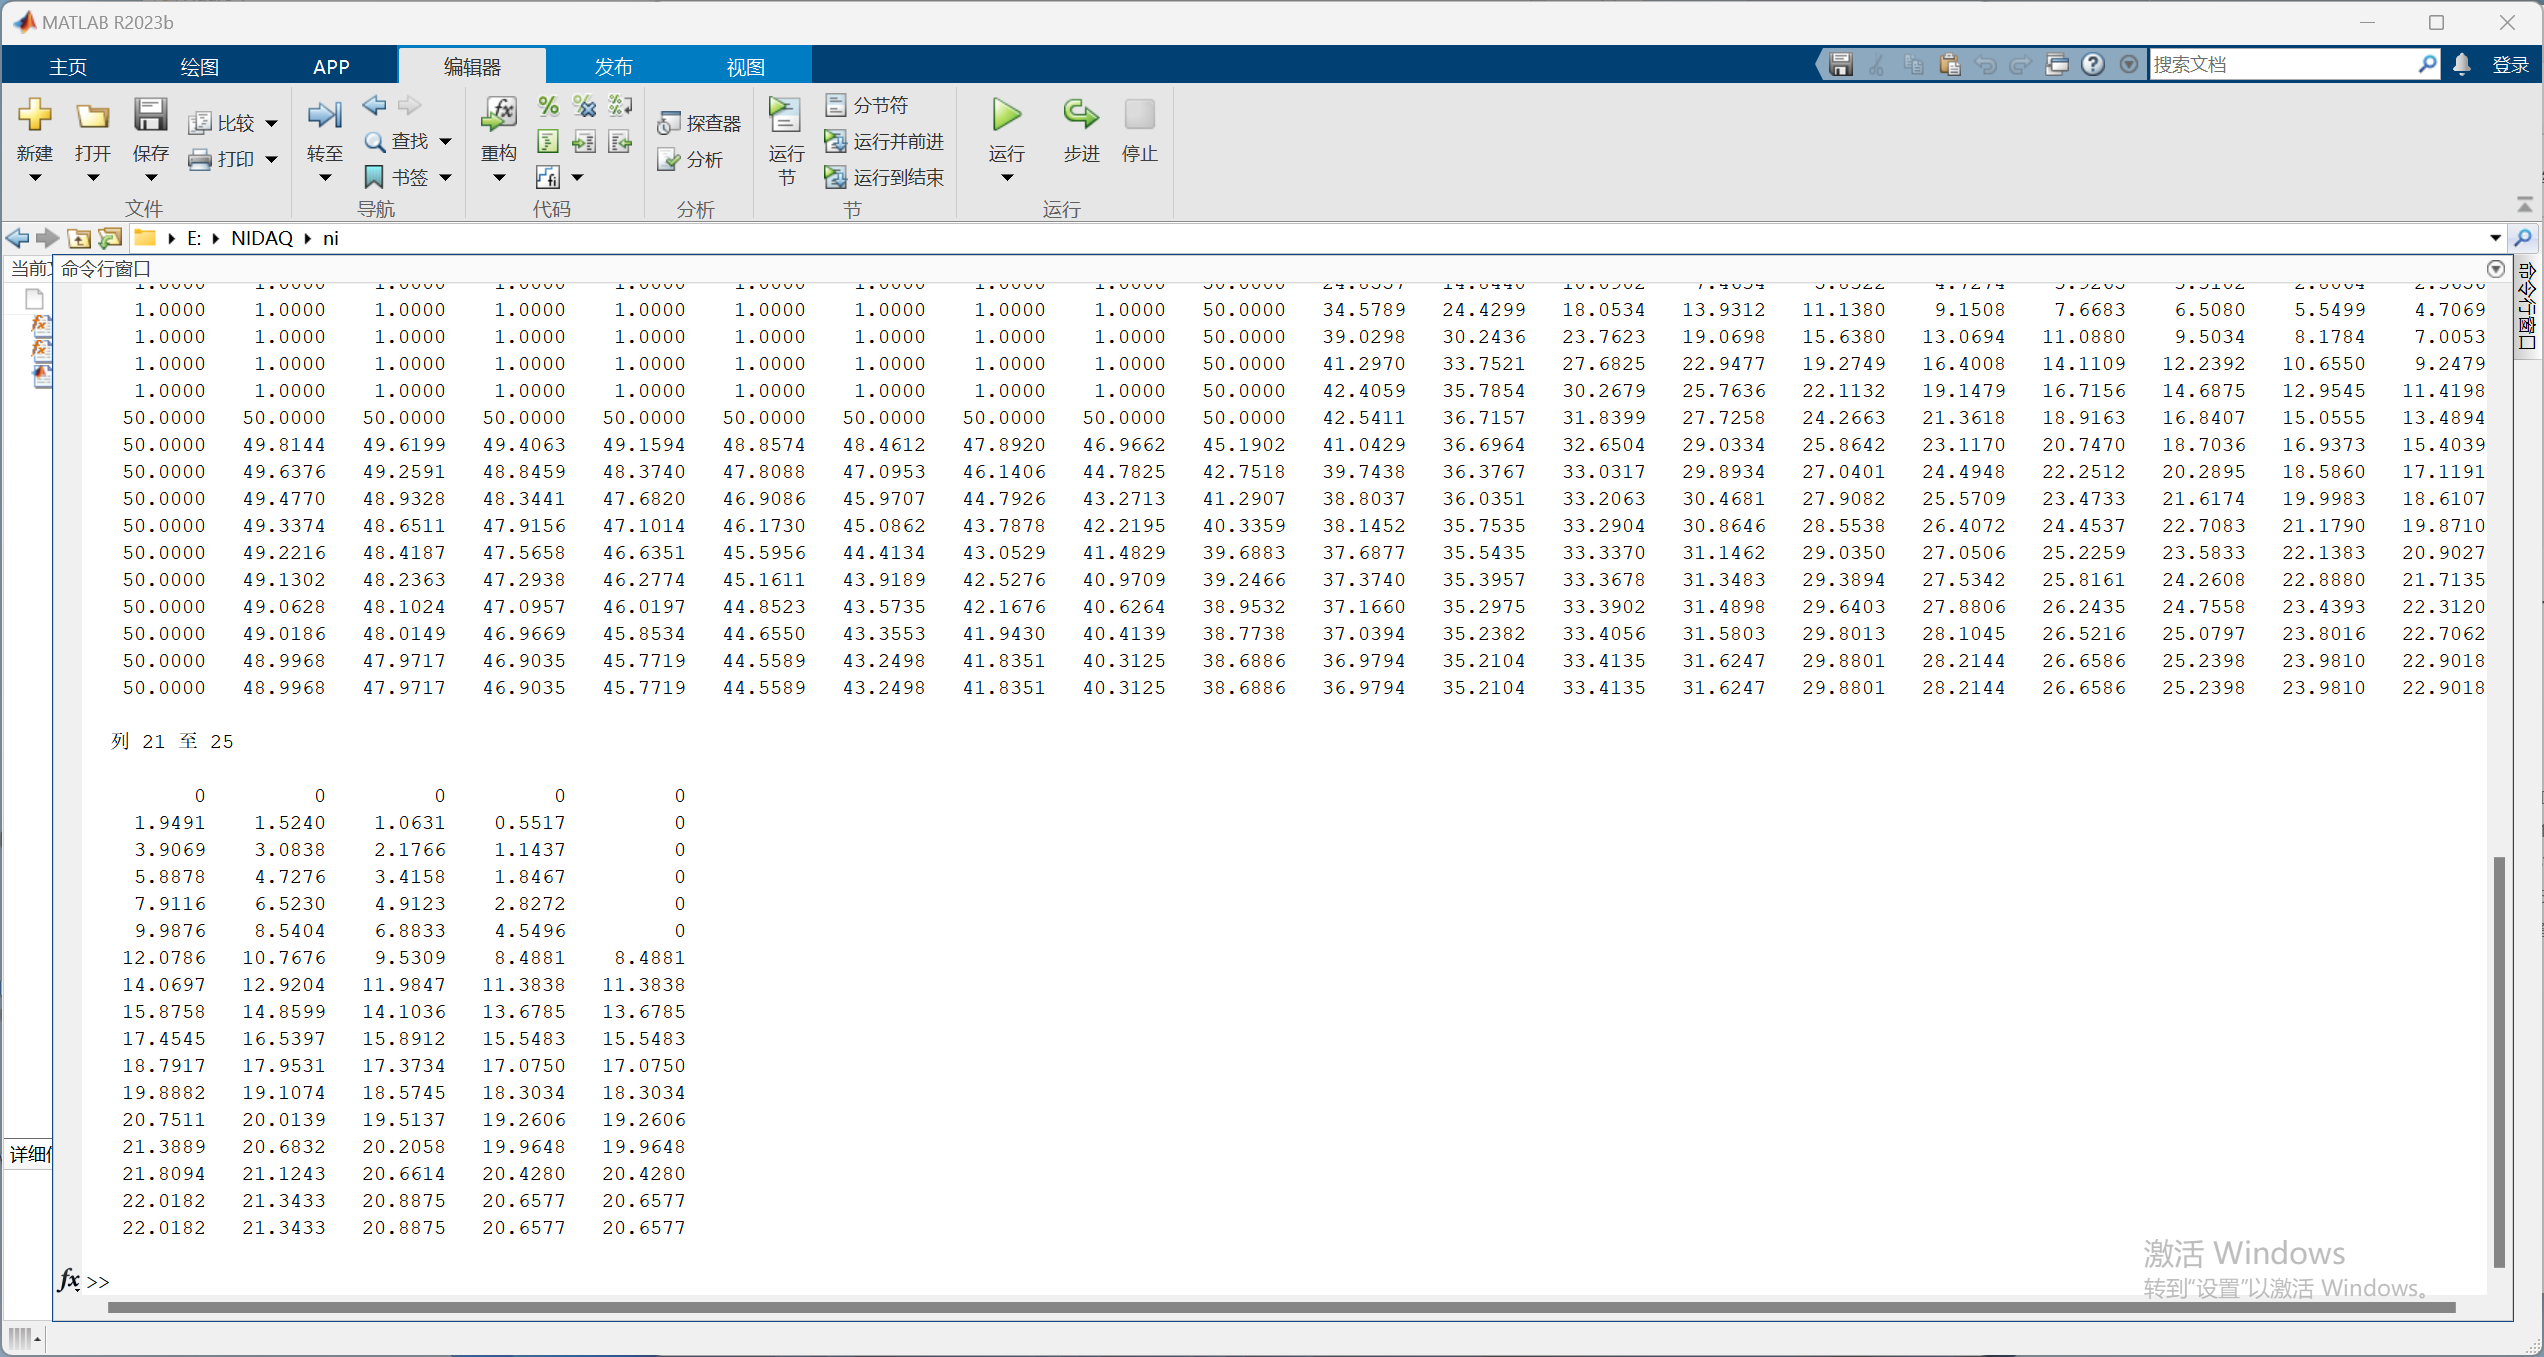
\includegraphics[width=0.85\textwidth]{数据4.png}
\end{center}

\end{document}